\subsection{Visão Estéreo}
    \label{subsec:intro_stereo}
A partir de duas ou mais imagens de um mesmo local (objeto ou até uma pessoa), é possível extrair, identificar e triangular suas características nas imagens e obter uma modelagem 3D; os problemas de~\emph{correspondência}~\cite{FergusL1}.

A priori a busca pelas correspondências ocorreria por toda a imagem; com uso das~\emph{linhas epipolares} reduz-se a uma busca linear. 
% Com base na Figura~\ref{fig:intro_stereo_epipolar_exemplo}, sabe-se
Sabe-se
que o ponto real $\mathbf{p}$ é representado pelos pontos $\mathbf{x_0}$ e $\mathbf{x_1}$ das imagens. Ao reprojetar linearmente o ponto $\mathbf{p}$ no infinito, $\mathbf{p_{\infty}}$, de modo a continuar sendo projetado no ponto $\mathbf{x_0}$ é possível determinar a linha epipolar a partir da diferença de projeção em relação a $\mathbf{x_1}$~\cite{Szeliski2012}.

% \begin{figure*}[!ht]
%     \begin{center}
%         \bmvaHangBox{\fbox{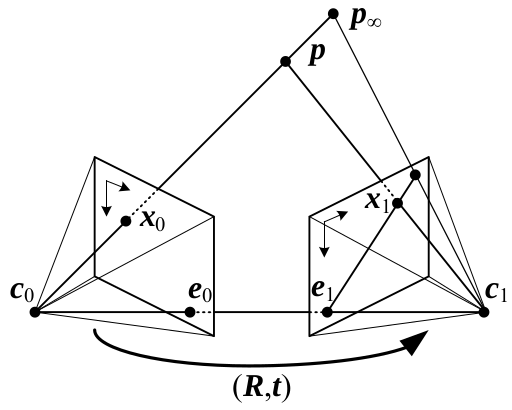
\includegraphics[width=3.8cm]{Figs/Introducao/linha_epipolar.png}}}
%     \end{center}
%     \caption{Representação visual da determinação de uma linha epipolar. Fonte~\cite{Szeliski2012}.}
%     \label{fig:intro_stereo_epipolar_exemplo}
% \end{figure*}

Com a aquisição das linhas epipolares de imagens correspondentes é possível reduzir a busca de correspondência numa linha horizontal, para alguns conjuntos de imagem~\cite{Szeliski2012}, 
% conforme ilustrado na Figura~\ref{fig:intro_stereo_match},
sendo denominado de~\emph{retificação}.

% \begin{figure}[!ht]
%     \centering
%     \begin{tabular}{cc}
%         \bmvaHangBox{\fbox{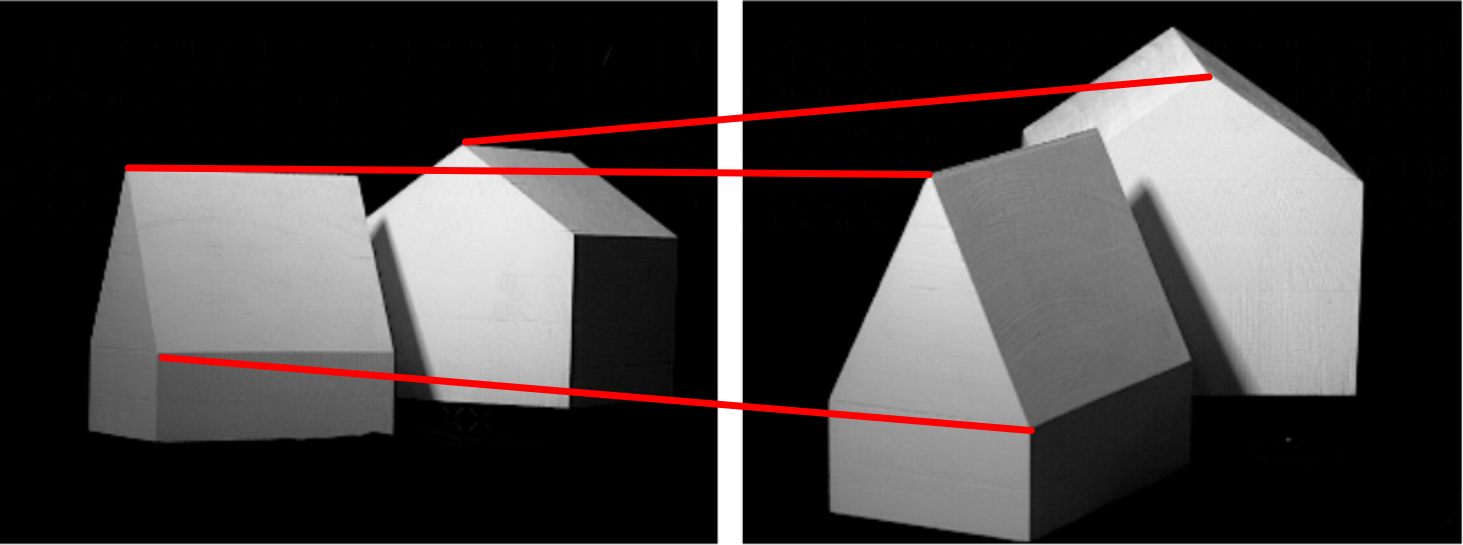
\includegraphics[height=1.5cm]{Figs/Introducao/original_stereo_.png}}}&
%         \bmvaHangBox{\fbox{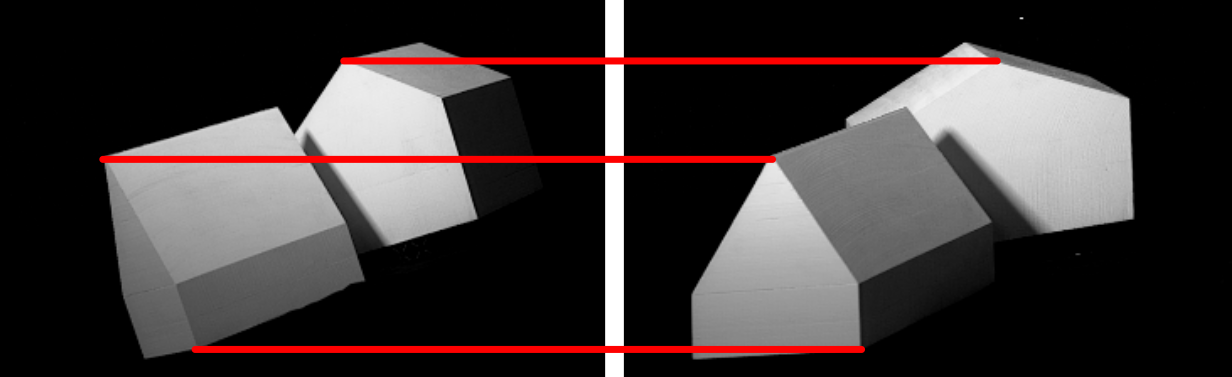
\includegraphics[height=1.5cm]{Figs/Introducao/ret_stereo_.png}}}\\
%         (a)&(b)
%     \end{tabular}
%     \caption{Retificação de um par de imagens estéreo, onde (a) são as imagens originais com linhas epipolares em diversas direções e (b) são as imagens retificação com todas as linhas epipolares na horizontal. Adaptado~\cite{Lazebnik1}.}
%     \label{fig:intro_stereo_match}
% \end{figure}

Além disso, a partir de duas imagens correspondentes a quantidade de movimentação que é percebida é denominada~\emph{disparidade}. Essa grandeza informa a distância entre os~\emph{pixels} correspondentes das imagens: $d_{(x, y)} = |x - x'| + |y - y'|$. Ao se calcular a disparidade para todos os~\emph{pixels} da imagem obtém-se seu~\emph{mapa de disparidade}
% , conforme ilustrado na Figura~\ref{fig:intro_stereo_disp_exemplo}
. No cenário de imagens correspondentes retificadas onde uma está certamente à direita da outra, a busca é ainda reduzida à esquerda do~\emph{pixel} base e vice-versa.

% \begin{figure}[!ht]
%     \centering
%     \begin{tabular}{cccc}
%         \bmvaHangBox{\fbox{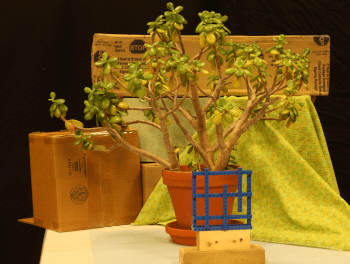
\includegraphics[width=3.3cm]{Figs/Introducao/exemplo_left.png}}}&
%         \bmvaHangBox{\fbox{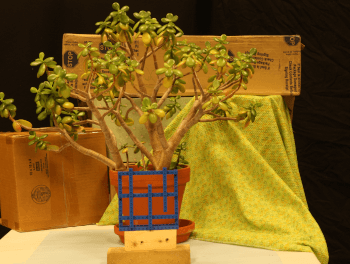
\includegraphics[width=3.3cm]{Figs/Introducao/exemplo_right.png}}}&
%         \bmvaHangBox{\fbox{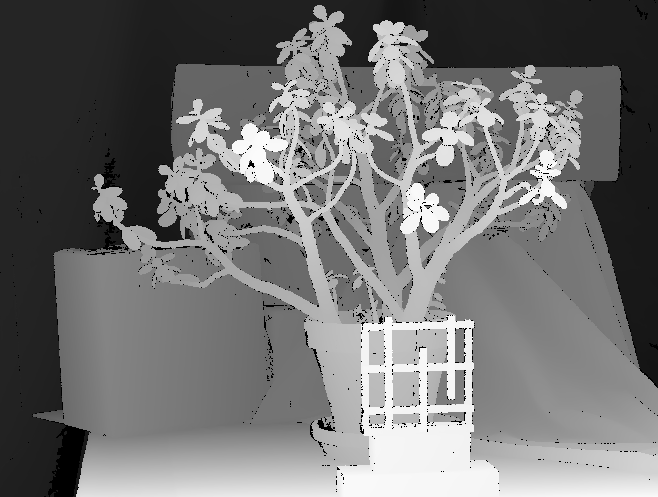
\includegraphics[width=3.3cm]{Figs/Introducao/exemplo_gt.png}}}\\
%         (a)&(b)&(c)
%     \end{tabular}
%     \caption{Mapa de disparidade para um par de imagens correspondentes retificadas, com as imagens exploradas por este trabalho. Têm-se os três componentes para esse mapa: (a) imagem base, (b) imagem correspondente à imagem base e (c) mapa de disparidade da imagem base.}
%     \label{fig:intro_stereo_disp_exemplo}
% \end{figure}

Com a aquisição do mapa de disparidade e em pose dos dados das câmeras (distância focal da imagem base $f$ e distância do mundo entre as câmeras $b$) é possível calcular o~\emph{mapa de profundidade}, uma vez que $Z_{xy} = (f \cdot b) /d_{xy}$.